\documentclass{report}
\usepackage[margin=1.3in]{geometry}
\usepackage{amssymb}
\usepackage{amsmath}
\usepackage{syntax}
\usepackage{pdfpages}

\usepackage[T1]{fontenc}
\usepackage{lmodern}
\begin{document}

\chapter{Appendix}
\section{Questionnaire Evaluation Materials}


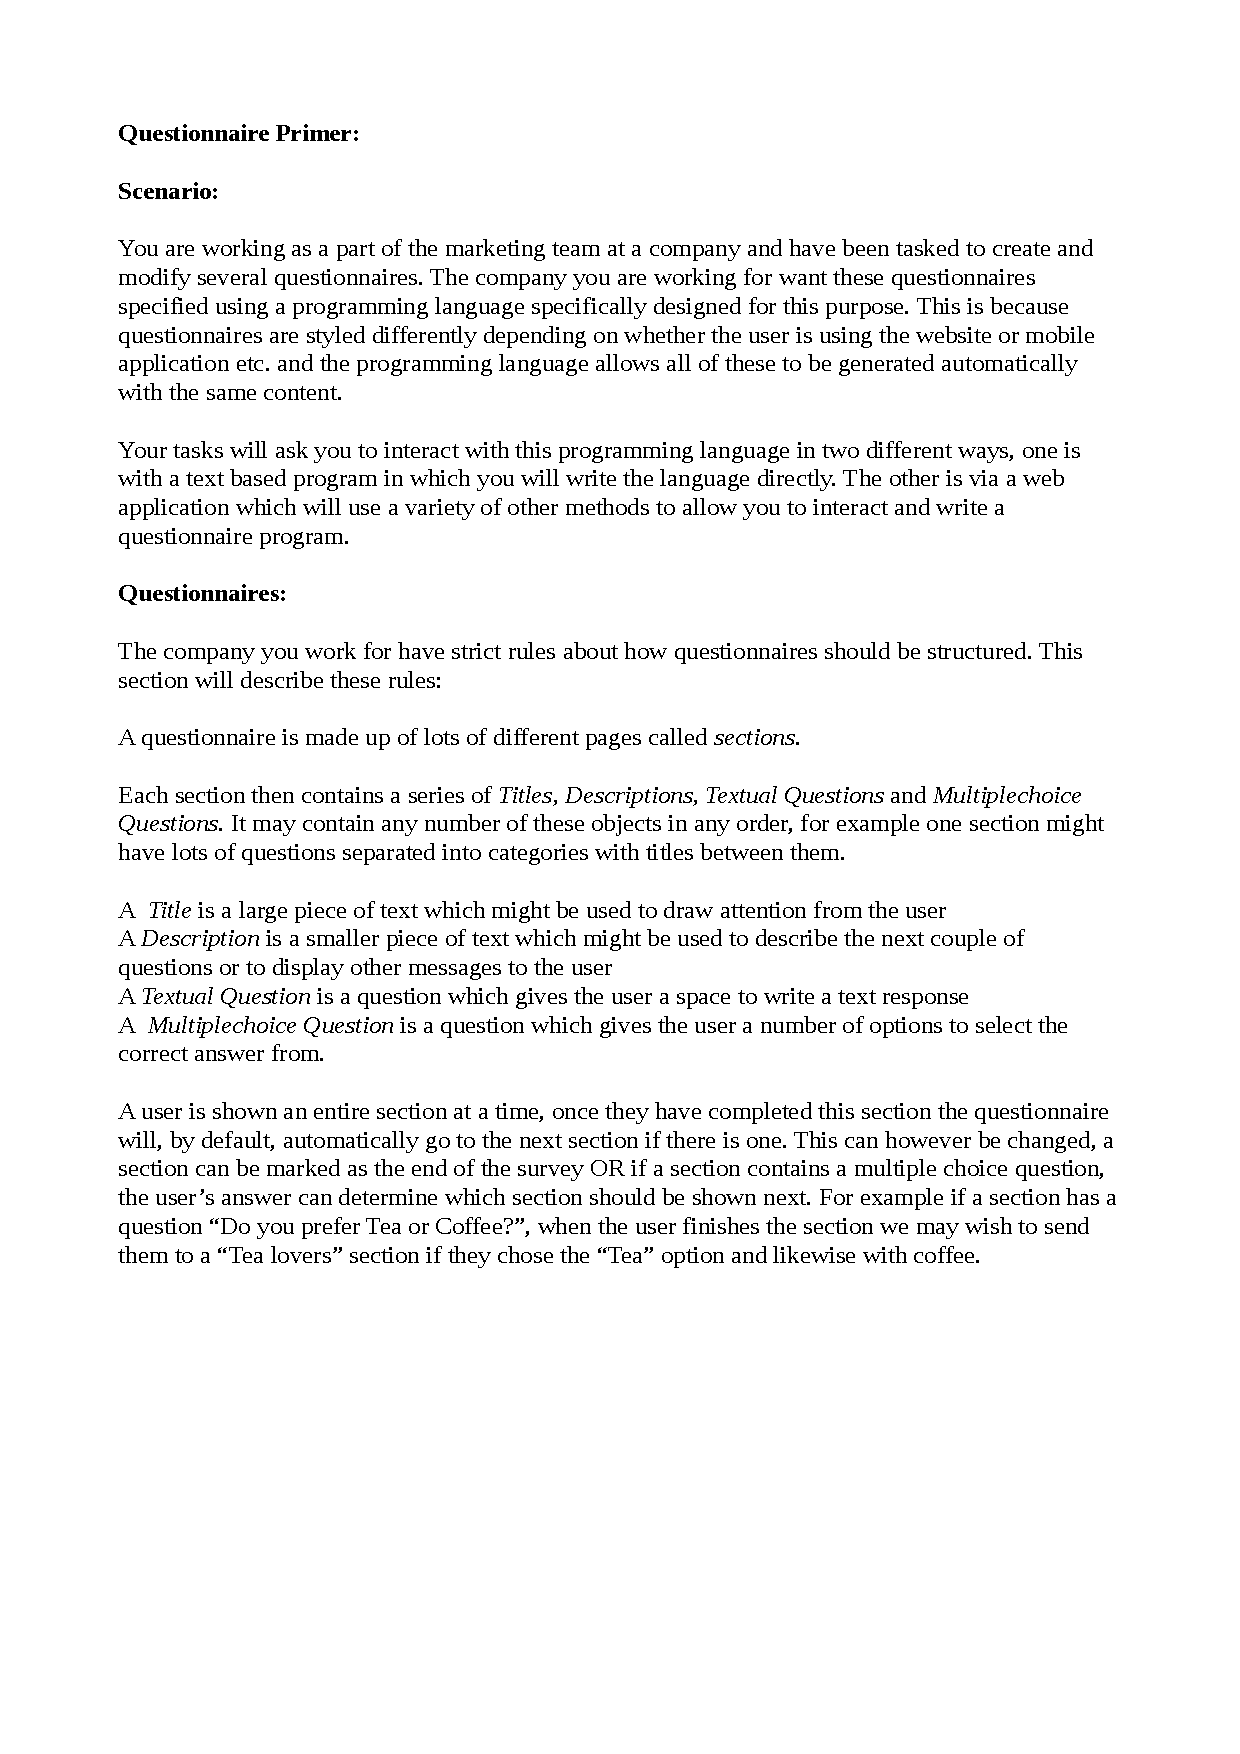
\includepdf[pages=1,scale=.8,pagecommand=\section{Training Material}]{./Appendix/QuestionnaireTraining.pdf}
\includepdf[pages=2-,scale=.8]{./Appendix/QuestionnaireTraining.pdf}

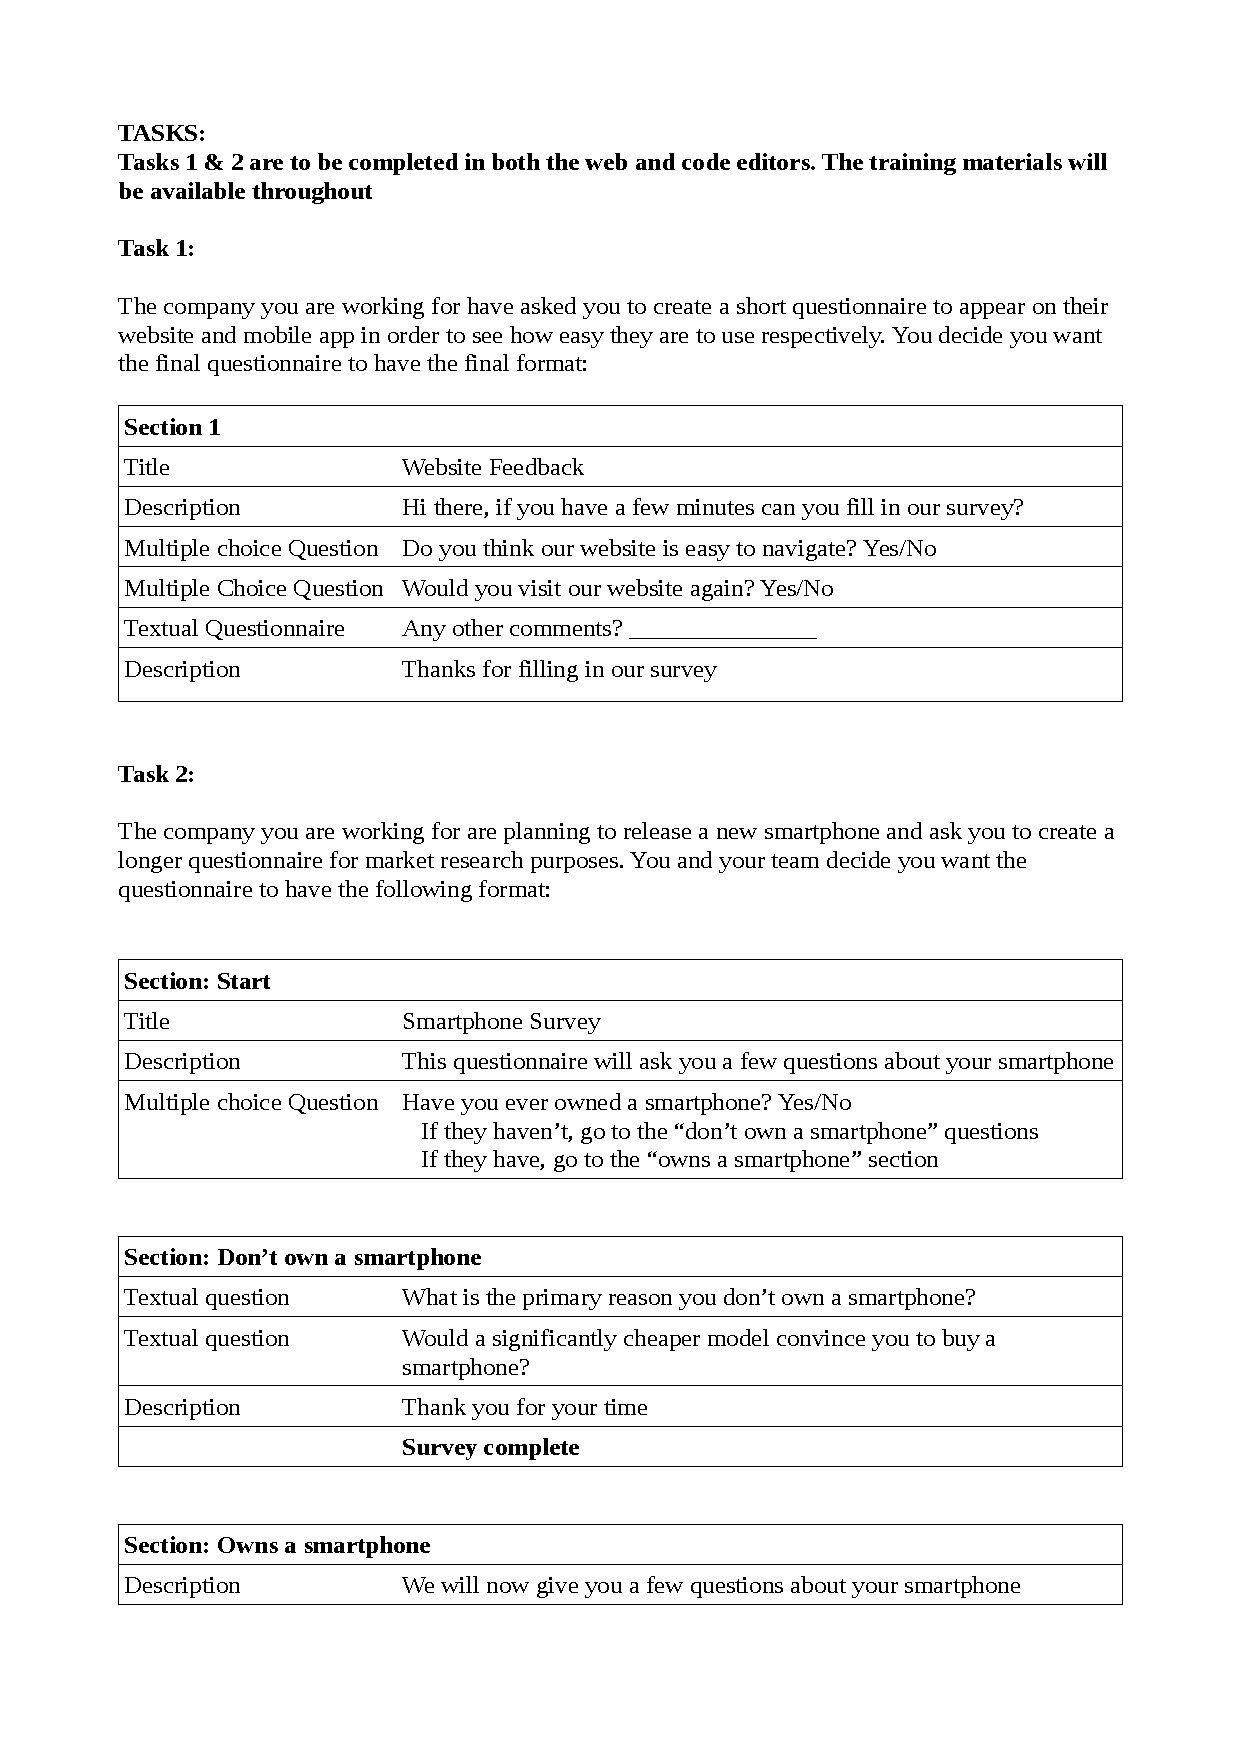
\includepdf[pages=1,scale=.8,pagecommand=\section{Task Sheet}]{./Appendix/QuestionnaireTasks.pdf}
\includepdf[pages=2-,scale=.8]{./Appendix/QuestionnaireTasks.pdf}

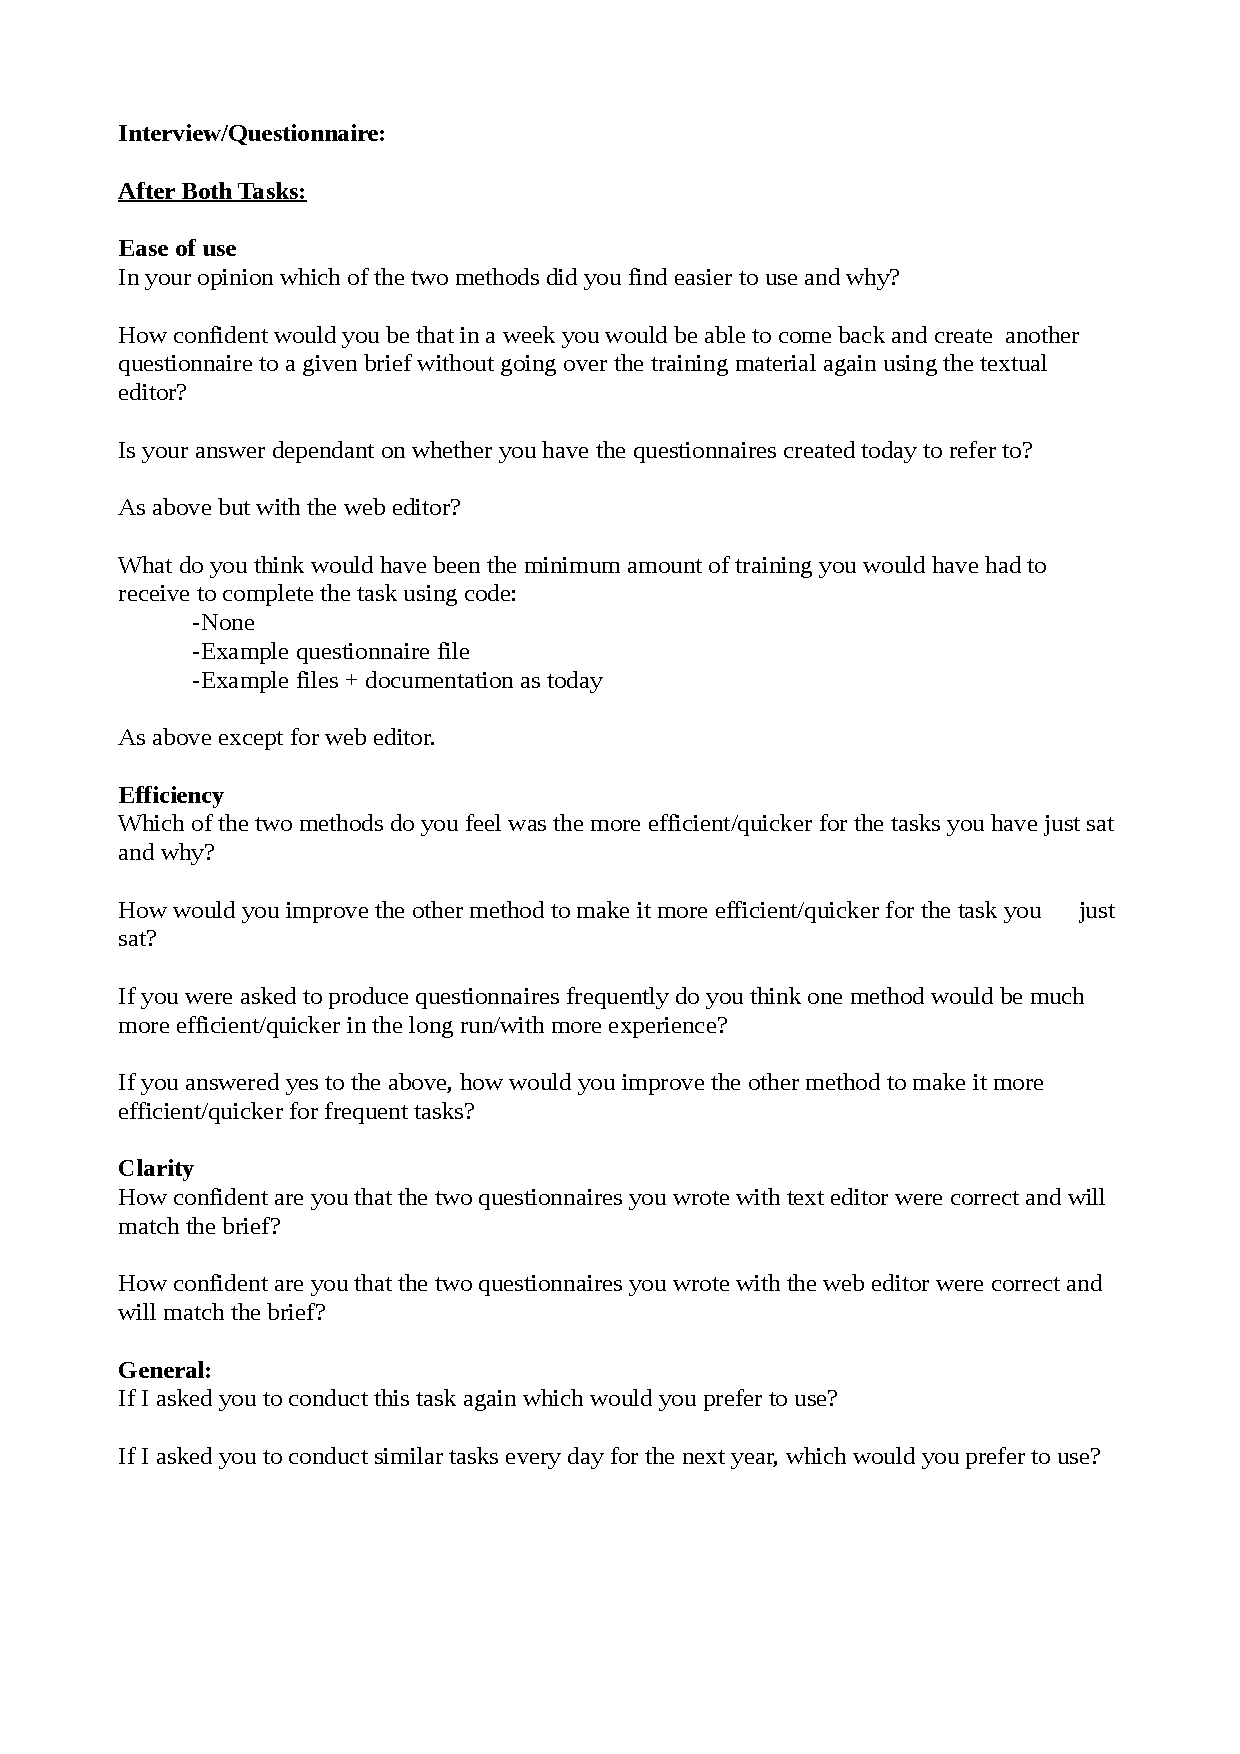
\includepdf[pages=-,scale=.8,pagecommand=\subsection{Interview Questions}]{./Appendix/InterviewQuestions.pdf}

\section{Questionnaire Evaluation Results}

\subsection{Respondant 1}
\subsubsection*{First editor used to complete tasks:} Eclipse
\subsubsection*{Times:}
\begin{itemize}
\item \emph{Eclipse Task 1:} 7:28
\item \emph{Eclipse Task 2:} 19:36
\item \emph{Web Task 1:} 2:35
\item \emph{Web Task 2:} 10:25
\end{itemize}
\subsubsection*{Observations made as completing tasks:}

\emph{Eclipse:}
\begin{itemize}
\item Significant confusion caused by curly brace positioning
\item Worried about spacing and initially spent a lot of time trying to perfectly match spaces in example/ training documentation
\item Missed string quotation marks
\item Found the error reporting in Eclipse difficult to deal with, despite positioning of red lines struggled to find where actual error was
\item Confusion from poorly named sections
\item Didn't make use of copy/paste in Android/iPhone section of 2nd task
\item Required help to finish task 2, couldn't work out brace positioning
\end{itemize}
\emph{Web Editor:}
\begin{itemize}
\item Didn't find adding extra sections not intuitive, got lost in tree view attempting to find
\item Tried to click on reference to section in main questionnaire view as if it were a link
\item Tried adding goto's to sections that didn't yet exist
\end{itemize}

\subsubsection*{Post Tasks Interview Transcript:}

\newpage
\subsection{Respondant 2}
\subsubsection*{First editor used to complete tasks:} Eclipse
\subsubsection*{Times:}
\begin{itemize}
\item \emph{Eclipse Task 1:} 4:24
\item \emph{Eclipse Task 2:} 17:05
\item \emph{Web Task 1:} 3:30
\item \emph{Web Task 2:} 11:03
\end{itemize}
\subsubsection*{Observations made as completing tasks:}

\emph{Eclipse:}
\begin{itemize}
\item Spent significant time during training looking at example file
\item Made use of copy and paste functionality to take structure from example file and modify the relevant fields
\item Unsure about spacing and asked several times if mattered
\item Struggled with curly braces
\item Made use of copy and paste within second task on Android/iPhone sections
\item Missed a curly brace, despite error underlining where it should be added and error message "Missing '\{'' " respondant assumed issue was elsewhere in the file and to do with spacing.
\end{itemize}
\emph{Web Editor:}
\begin{itemize}
\item Found confusing had to add section before could cross reference
\item Did use the sub tree views to modify just a particular question
\end{itemize}

\subsubsection*{Post Tasks Interview Transcript:}

\newpage
\subsection{Respondant 3}
\subsubsection*{First editor used to complete tasks:} Web
\subsubsection*{Times:}
\begin{itemize}
\item \emph{Eclipse Task 1:} 4:03
\item \emph{Eclipse Task 2:} 15:14
\item \emph{Web Task 1:} 3:19
\item \emph{Web Task 2:} 10:57
\end{itemize}
\subsubsection*{Observations made as completing tasks:}

\emph{Eclipse:}
\begin{itemize}
\item Missed 'Section' keyword when creating first section in task 1 and had some difficulty in realising this was the cause of an error as the produced error message wasn't clear. Saying only "EOF was expected"
\item Made use of copy and paste on individual questions, modifying relevant attributes only
\item Had little issue with curly braces, perhaps as made use of Eclipse's automatic insertion of these
\end{itemize}
\emph{Web Editor:}
\begin{itemize}
\item Struggled with navigating between questionnaire editor and section editor at first
\item Confusion caused by adding nodes which are generated from the parse tree but in themselves are meaningless, normally only used for other nodes to inherit
\item Tried clicking on references in questionnaire editor
\item Tried adding references in goto feature despite references not yet existing.
\end{itemize}

\subsubsection*{Post Tasks Interview Transcript:}



\end{document}